\documentclass{article}
\usepackage{enumerate}
\usepackage{amsmath}
\usepackage{amssymb}
\usepackage{graphicx}
\usepackage{subfigure}
\usepackage{geometry}
\usepackage{caption}
\usepackage{indentfirst}
\usepackage{tikz}
\usetikzlibrary{circuits.logic.US}
\usetikzlibrary{arrows.meta}
\usetikzlibrary{calc}
\geometry{left=3.0cm,right=3.0cm,top=3.0cm,bottom=3.0cm}
\renewcommand{\thesection}{Problem \arabic{section}.}
\title{VE270 Homework 6}
\author{Liu Yihao 515370910207}
\date{}

\newcommand{\drawmuxtwo}[3]{
	\draw #1 node (#2) [shape=rectangle,draw,minimum height=2cm,minimum width=2cm,text width=1cm,align=center] {#3};
	\draw (#2) ++(down:7.5mm) node {$s_0$};
	\draw (#2) ++(right:7.5mm) node {$d$};
	\draw (#2) ++(left:7.5mm) ++(up:2.5mm) node {$i_0$} ++(down:5mm) node {$i_1$};
}
\newcommand{\drawmuxfour}[3]{
	\draw #1 node (#2) [shape=rectangle,draw,minimum height=3cm,minimum width=2cm,text width=1cm,align=center] {#3};
	\draw (#2) ++(left:7.5mm) ++(up:7.5mm) node {$i_0$} ++(down:5mm) node {$i_1$} ++(down:5mm) node {$i_2$} ++(down:5mm) node {$i_3$};
	\draw (#2) ++(down:12.5mm)++(left:3.33mm) node {$s_1$} ++(right:6.66mm) node {$s_0$};
	\draw (#2) ++(right:7.5mm) node {$d$};
}
\newcommand{\drawmuxeight}[3]{
	\draw #1 node (#2) [shape=rectangle,draw,minimum height=5cm,minimum width=2cm,text width=1cm,align=center] {#3};
	\draw (#2) ++(left:7.5mm) ++(up:17.5mm) node {$i_0$} ++(down:5mm) node {$i_1$} ++(down:5mm) node {$i_2$} ++(down:5mm) node {$i_3$} ++(down:5mm) node {$i_4$} ++(down:5mm) node {$i_5$} ++(down:5mm) node {$i_6$} ++(down:5mm) node {$i_7$};
	\draw (#2) ++(down:22.5mm) node {$s_1$} ++(left:5mm) node {$s_2$} ++(right:10mm) node {$s_0$};
	\draw (#2) ++(right:7.5mm) node {$d$};
}
\newcommand{\drawdecodereight}[3]{
	\draw #1 node (#2) [shape=rectangle,draw,minimum height=5cm,minimum width=2cm,text width=1cm,align=center] {#3};
	\draw (#2) ++(right:7.5mm) ++(up:17.5mm) node {$d_0$} ++(down:5mm) node {$d_1$} ++(down:5mm) node {$d_2$} ++(down:5mm) node {$d_3$} ++(down:5mm) node {$d_4$} ++(down:5mm) node {$d_5$} ++(down:5mm) node {$d_6$} ++(down:5mm) node {$d_7$};
	\draw (#2) ++(left:7.5mm) node {$i_1$} ++(up:5mm) node {$i_0$} ++(down:10mm) node {$i_2$};
}
\newcommand{\drawfulladder}[3]{
	\draw #1 node (#2) [shape=rectangle,draw,minimum height=2cm,minimum width=2cm,text width=1cm,align=center] {#3};
	\draw (#2) ++(left:7.5mm) node {$c_o$};
	\draw (#2) ++(right:7.5mm) node {$c_i$};
	\draw (#2) ++(down:7.5mm) node {$s$};
	\draw (#2) ++(up:7.5mm) ++(left:3.3mm) node {$a$} ++(right:6.6mm) node {$b$};
}

\newcommand{\drawaddermodel}[3]{
	\draw #1 node (#2) [shape=rectangle,draw,minimum height=2cm,minimum width=4cm,text width=3cm,align=center] {#3};
	\draw (#2) ++(left:17.5mm) node {$c_o$};
	\draw (#2) ++(right:17.5mm) node {$c_i$};
	\draw (#2) ++(down:7.5mm) node {$s$};
	\draw (#2) ++(up:7.5mm) ++(left:10mm) node {$a$} ++(right:20mm) node {$b$};
}

\newcommand{\drawadder}[4]{
	\drawaddermodel{#1}{#2}{#3}
	\draw (#2) ++(up:10mm) ++(left:10mm) to node {$\diagup$} node[left] {8} ++(up:10mm) ;
	\draw (#2) ++(up:10mm) ++(right:10mm) to node {$\diagup$} node[left] {8} ++(up:10mm) ;
}

\newcommand{\drawsubtractor}[4]{
	\drawaddermodel{#1}{#2}{#3}
	\draw (#2) ++(up:10mm) ++(left:10mm) to node {$\diagup$} node[left] {8} ++(up:20mm);
	\draw (#2) ++(up:21.5mm) ++(right:10mm) node[not gate,point down] (#2__notgate) {#4 bit};
	\draw (#2) ++(up:10mm) ++(right:10mm) to node {$\diagup$} node[left] {#4} (#2__notgate.output);
	\draw (#2) ++(up:30mm) ++(right:10mm) to node {$\diagup$} node[left] {#4} (#2__notgate.input);
}


\begin{document}
\maketitle

\section{}
\begin{center}
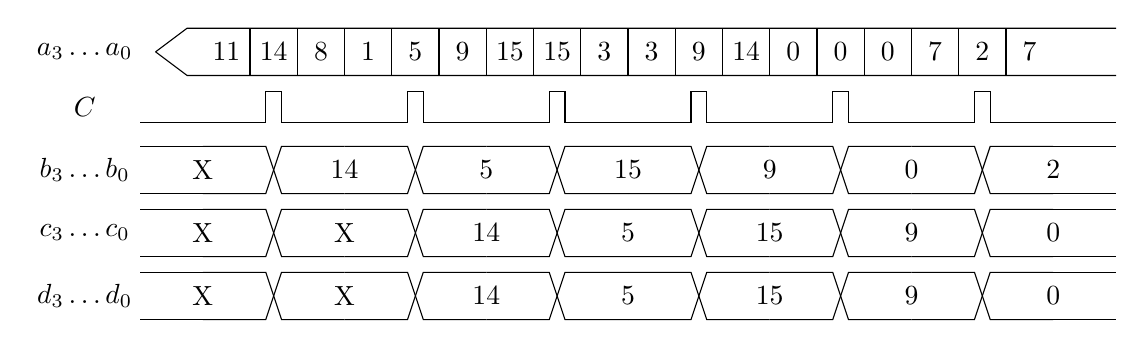
\begin{tikzpicture}[scale=0.8]
	\foreach \i/\val in {1/11,2/14,3/8,4/1,5/5,6/9,7/15,8/15,9/3,10/3,11/9,12/14,13/0,14/0,15/0,16/7,17/2,18/7} {
		\draw (\i*0.75,0) node {\val};
		\ifnum \i<18
			\draw (\i*0.75+0.375,0.375) -- ++(down:7.5mm);
		\fi
	};
	\draw (14.875,0.375) -- (0.125,0.375) -- (-0.375,0);
	\draw (14.875,-0.375) -- (0.125,-0.375) -- (-0.375,0);
	\foreach \i in {0,...,5} {
		\draw (3*0.75*\i+0.375,-1.5+0.375) -- ++(right:1cm) -- ++(up:5mm) -- ++(right:2.5mm) -- ++(down:5mm) -- ++(right:1cm);
	};
	\draw (0.375,-1.5+0.375) -- ++(left:1cm) (13.875,-1.5+0.375) -- ++(right:1cm);
	\foreach \j in {0,1,2} {
		\foreach \i in {0,...,5} {
			\draw (3*0.75*\i+0.375,-1.5-\j) -- ++(right:1cm) -- ++($(right:2.5mm)+(down:7.5mm)$) -- ++(right:1cm);
			\draw (3*0.75*\i+0.375,-2.25-\j) -- ++(right:1cm) -- ++($(right:2.5mm)+(up:7.5mm)$) -- ++(right:1cm);
		};
		\draw (0.375,-1.5-\j) -- ++(left:1cm) (13.875,-1.5-\j) -- ++(right:1cm);
		\draw (0.375,-2.25-\j) -- ++(left:1cm) (13.875,-2.25-\j) -- ++(right:1cm);
	};
	\foreach \i/\val in {0/X,1/14,2/5,3/15,4/9,5/0,6/2}
		\draw (3*0.75*\i+0.375,-1.875) node {\val};
	\foreach \i/\val in {0/X,1/X,2/14,3/5,4/15,5/9,6/0} {
		\draw (3*0.75*\i+0.375,-2.875) node {\val};
		\draw (3*0.75*\i+0.375,-3.875) node {\val};
	};
	\draw (-1.5,0) node {$a_3\dots a_0$};
	\draw (-1.5,-0.875) node {$C$};
	\draw (-1.5,-1.875) node {$b_3\dots b_0$};
	\draw (-1.5,-2.875) node {$c_3\dots c_0$};
	\draw (-1.5,-3.875) node {$d_3\dots d_0$};
\end{tikzpicture}
\end{center}

\section{}
\begin{center}
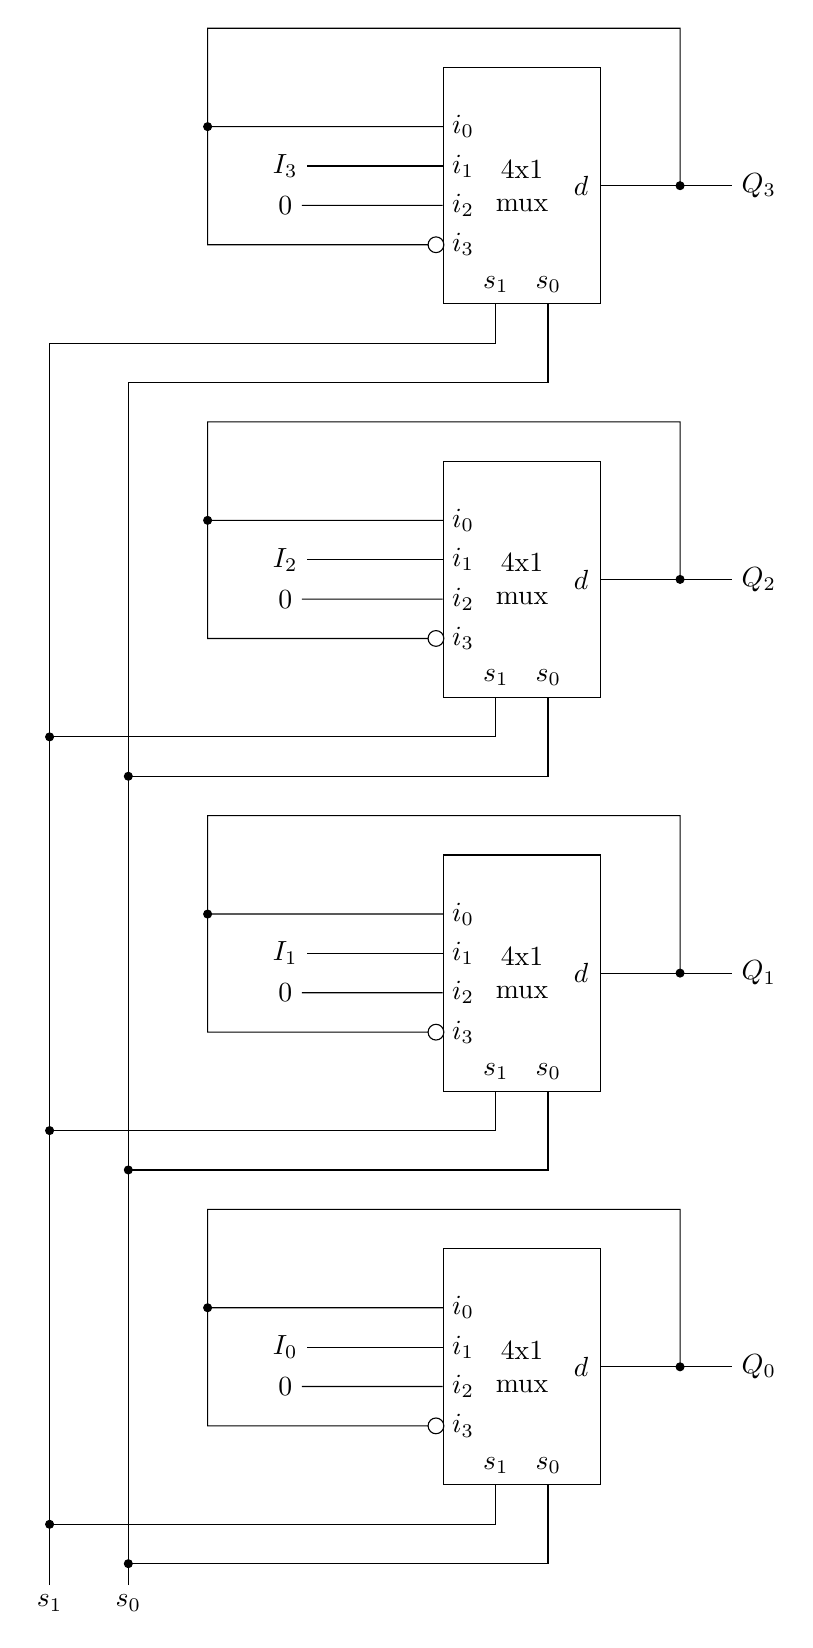
\begin{tikzpicture}[circuit logic US]
\draw (-5,-3) node (s0) {$s_0$};
\draw (-6,-3) node (s1) {$s_1$};
\draw (s0) -- (-5,12.5);
\draw (s1) -- (-6,13);
\foreach \i in {0,...,3} {
	\drawmuxfour{(0,5*\i)}{m\i}{4x1 mux};
	\draw (m\i.east) ++(right:2cm) node (Q\i) {$Q_\i$};
	\draw (m\i.east) -- (Q\i);
	\filldraw (m\i.east) ++(right:1cm) circle [radius=0.5mm];
	\filldraw (m\i.east) ++(left:5cm) ++(up:0.75cm) circle [radius=0.5mm];
	\draw (m\i.east) ++(right:1cm) -- ++(up:2cm) -- ++(left:6cm) -- ++(down:1.25cm) -- ++(right:3cm) ++(left:3cm) -- ++(down:1.5cm) -- ++(right:2.8cm) ++(right:1mm) circle [radius=1mm];
	\draw (m\i.west) ++(up:2.5mm) ++(left:2cm) node (I\i) {$I_\i$} ++(down:5mm) node (g\i) {0};
	\draw (m\i.west) ++(up:2.5mm) -- (I\i);
	\draw (m\i.west) ++(down:2.5mm) -- (g\i);
	\draw (s0) ++(up:5*\i+0.5) -- ++(right:5.33cm) -- ++(up:1cm);
	\draw (s1) ++(up:5*\i+1) -- ++(right:5.66cm) -- ++(up:0.5cm);
	\ifnum \i<3
		\filldraw (s0) ++(up:5*\i+0.5) circle [radius=0.5mm];
		\filldraw (s1) ++(up:5*\i+1) circle [radius=0.5mm];
	\fi
a};
\end{tikzpicture}
\end{center}

\section{}
\begin{center}
\begin{tikzpicture}[circuit logic US]
	\foreach \i/\j/\n in {0/1/c,1/2/b,2/4/a} {
		\drawshifter{(0,2*\i)}{s\i}{$<<\j$}{16};
		\draw (s\i.west) ++(left:1.5cm) node (\n) {\n};
		\draw (\n) -- (s\i.west);
		\draw (s\i.east) ++(right:1.5cm) node (g\i) {0};
		\draw (g\i) -- (s\i.east);
	};
	\draw (s2.north) ++(up:1.5cm) node (I) {I};
	\draw (s0.south) ++(down:1.5cm) node (Q) {Q};
	\draw (s2.north) -- (I) (s0.south) -- (Q);
\end{tikzpicture}
\end{center}

\section{}
\begin{enumerate}[(a)]
\item \
\begin{center}
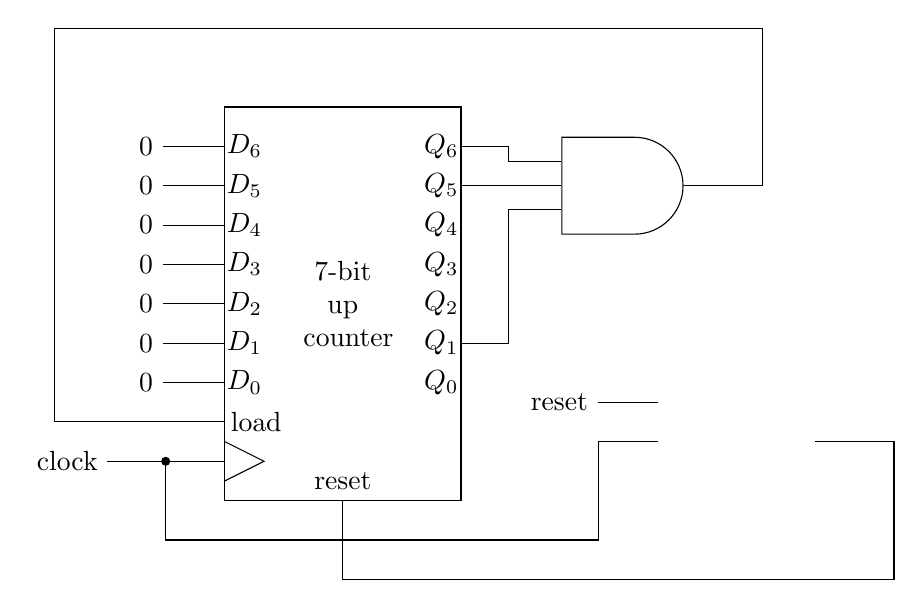
\begin{tikzpicture}[circuit logic US]
	\draw (0,0) node (c) [draw,shape=rectangle,minimum height=5cm,minimum width=3cm,text width=1cm,align=center] {7-bit up counter};
	\foreach \i in {0,...,6} {
		\draw (c) ++(left:1.25cm) ++(up:0.5*\i-1) node {$D_\i$};
		\draw (c) ++(right:1.25cm) ++(up:0.5*\i-1) node {$Q_\i$};
		\draw (c) ++(left:2.5cm) ++(up:0.5*\i-1) node (g\i) {0};
		\draw (c) ++(left:1.5cm) ++(up:0.5*\i-1) -- (g\i);
	};
	\draw (c) ++(left:1.1cm) ++(down:1.5) node {load};
	\draw (c) ++(left:1.5cm) ++(down:1.75) -- ++($(right:5mm)+(down:2.5mm)$) -- ++($(left:5mm)+(down:2.5mm)$);
	\draw (c) ++(down:2.25cm) node {reset};
	\draw (3.5,1.5) node (g) [and gate,scale=2,inputs=nnn] {};
	\draw (1.5,2) -- ++(right:6mm) |- (g.input 1);
	\draw (1.5,1.5) -- (g.input 2);
	\draw (1.5,-0.5) -- ++(right:6mm) |- (g.input 3);
	\draw (g.output) -- ++(right:1cm) -- ++(up:2cm) -- ++(left:9cm) |- (-1.5,-1.5);
	\drawdflipflop{(5,-1.5)}{dfp}{D flip flop};
	\draw (2.75,-1.25) node (rst) {reset};
	\draw (rst) -- (4,-1.25);
	\draw (-3.5,-2) node (clk) {clock};
	\draw (clk) -- (-1.5,-2);
	\filldraw (-2.25,-2) circle [radius=0.5mm];
	\draw (-2.25,-2) -- ++(down:1cm) -- ++(right:5.5cm) |- (4,-1.75);
	\draw (6,-1.75) -- ++(right:1cm) -- ++(down:1.75cm) -| (0,-2.5);
\end{tikzpicture}
\end{center}
\item \
\begin{center}
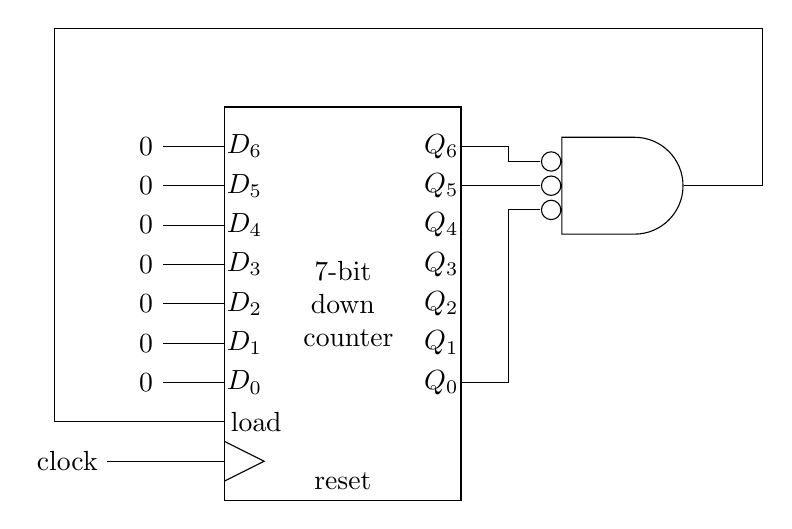
\begin{tikzpicture}[circuit logic US]
	\draw (0,0) node (c) [draw,shape=rectangle,minimum height=5cm,minimum width=3cm,text width=1cm,align=center] {7-bit down counter};
	\foreach \i in {0,...,6} {
		\draw (c) ++(left:1.25cm) ++(up:0.5*\i-1) node {$D_\i$};
		\draw (c) ++(right:1.25cm) ++(up:0.5*\i-1) node {$Q_\i$};
		\draw (c) ++(left:2.5cm) ++(up:0.5*\i-1) node (g\i) {0};
		\draw (c) ++(left:1.5cm) ++(up:0.5*\i-1) -- (g\i);
	};
	\draw (c) ++(left:1.1cm) ++(down:1.5) node {load};
	\draw (c) ++(left:1.5cm) ++(down:1.75) -- ++($(right:5mm)+(down:2.5mm)$) -- ++($(left:5mm)+(down:2.5mm)$);
	\draw (c) ++(down:2.25cm) node {reset};
	\draw (3.5,1.5) node (g) [and gate,scale=2,inputs=iii] {};
	\draw (1.5,2) -- ++(right:6mm) |- (g.input 1);
	\draw (1.5,1.5) -- (g.input 2);
	\draw (1.5,-1) -- ++(right:6mm) |- (g.input 3);
	\draw (g.output) -- ++(right:1cm) -- ++(up:2cm) -- ++(left:9cm) |- (-1.5,-1.5);
	\draw (-3.5,-2) node (clk) {clock};
	\draw (clk) -- (-1.5,-2);
\end{tikzpicture}
\end{center}
\end{enumerate}

\section{}
\begin{center}
\begin{tikzpicture}[circuit logic US]
	\drawshiftreg{(0,0)}{s}{8-bit shift register}{8};
	\drawregister{(0,-3)}{r}{8-bit register RxReg}{8};
	\draw (-7.5,-3) node (c) [draw,shape=rectangle,minimum height=2cm,minimum width=3cm,text width=2cm,align=center] {3-bit up counter};
	\draw (c) ++(down:7.5mm) node {reset};
	\draw (c) ++(right:12.5mm) ++(down:5mm) node {$Q_0$};
	\draw (c) ++(right:12.5mm) node {$Q_1$};
	\draw (c) ++(right:12.5mm) ++(up:5mm) node {$Q_2$};
	\draw (c) ++(left:11.54mm) -- ++($(left:3.46mm)+(down:2mm)$);
	\draw (c) ++(left:11.54mm) -- ++($(left:3.46mm)+(up:2mm)$);
	\draw (-4,-3) node (g) [and gate,scale=2,inputs=nnn] {};
	\draw (g.output) -- (r.west);
	\filldraw (g.output) ++(right:7.5mm) circle [radius=0.5mm];
	\draw (g.output) ++(right:7.5mm) -- ++(down:1.5cm) -| (c.south);	
	\draw (c.east) ++(up:5mm) -- ++(right:5mm) |- (g.input 1);
	\draw (c.east) -- (g.input 2);
	\draw (c.east) ++(down:5mm) -- ++(right:5mm) |- (g.input 3);
	\draw (-11,0) node (valid) {Valid};
	\draw (valid) -- (s.west);
	\filldraw (valid) ++(right:1cm) circle [radius=0.5mm];
	\draw (valid) ++(right:1cm) |- (c.west);
	\draw (3,0) node (in) {Data\_in};
	\draw (in) -- (s.east);
\end{tikzpicture}
\end{center}






\end{document}
